\subsection{\label{sec:A1}Dark field microscopy}
Before delving into the qualitative analysis of the captured sample images, 
we provide a detailed description of the adjustment process. 
Initially, the sample must be shifted into the focus of the first objective. 
This adjustment is achieved by finely manipulating the sample stage using small knobs, 
allowing precise movement in all three spatial directions. 
The light reflected from the sample is directed onto the adjustable camera via a beam splitter, 
positioned above the light source for this initial step. 
The sample stage is finely adjusted until the nanorod sample fields are distinctly visible 
in sharp focus on the transmitted image. \\
Subsequently, the camera can be relocated to the position shown 
in Fig.~\ref{fig:aufbau}. 
In this configuration, the camera captures the light transmitted through the sample. 
The rear objective is adjusted to render the displayed image sharp. 
As a result, the sample is now in focus for both objectives. \\
At this point, a dark-field mask can be introduced into the optical path, 
preventing excitation light from reaching the second objective. 
Nevertheless, a signal corresponding to the scattered light from the nanoparticles is still 
detected on the camera. 
By inserting a polarizer, the unpolarized light can be linearly polarized, 
with the option of aligning it parallel or perpendicular to the nanorods, 
corresponding to settings of $0^{\circ}$ or $90^{\circ}$. \\ \\
Initially, images are captured in bright-field and dark-field modes without a polarizer. 
The recordings are depicted in Fig.~\ref{fig:bilder}.
\begin{figure}[h!]
    \centering
    \subfloat[\centering Bright-field image]{{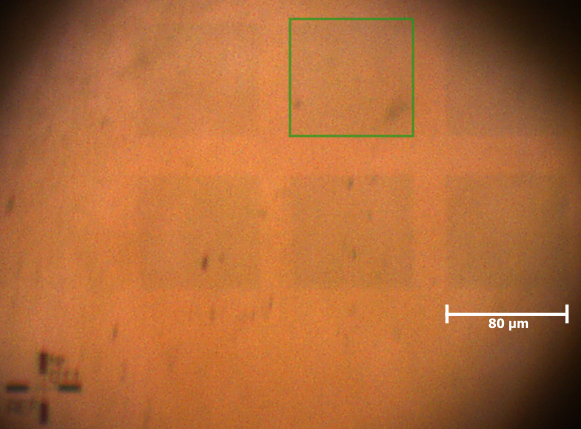
\includegraphics[width=0.47\textwidth]{Hell.png} }}
    \qquad
    \subfloat[\centering Dark-field image]{{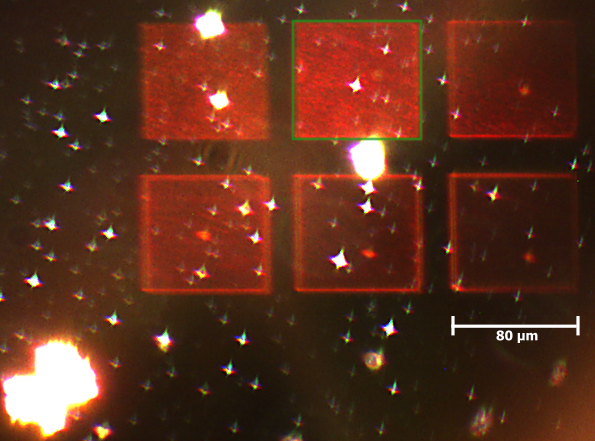
\includegraphics[width=0.47\textwidth]{DunkelBild.png} }}
    \caption{\label{fig:bilder}An image of the sample in bright-field mode, depicting light transmitted 
    through the sample (a), and in dark-field mode, illustrating light scattered by the sample (b). 
    The excitation light is non-polarized. A reference marker in the bottom left corner confirms 
    observation of the same areas of the sample.
    Additionally, a sample field has been marked in green, serving as a guide to the eye.}
\end{figure}\FloatBarrier 